\graphicspath{{chapters/08/images/}}
\chapter{Scaffold design}

\section{Introduction}
Tissue engineering is the 3D assembly over time of vital tissues-organs by a process involving cells, signals, and the extracellular matrix.
The dynamics of regeneration vary from tissue to tissue according to the hierarchy of tissue or organ function.

    \subsection{Material design}
    A biocompatible material must have the ability to perform a specific application with an appropriate host response.
    The main consideration to be made when designing a material are:

    \begin{multicols}{2}
        \begin{itemize}
            \item sourcing of functional cells: if the scaffold requires a pre-loading of cells, the type of cell needed and where to obtain them need to be decided.
            \item GF regulatory systems: synthetic polymers with no biorecognition properties require functionalization>
            \item immuno acceptance:  for example force stem cells to become osteoblasts or modulate the immune response in order to shorten the inflammation and boost regeneration.
        \end{itemize}
    \end{multicols}

    Biological information is required for performing in vitro tests and for functionalization that needs to be linked to specific biological pathways and is essential to thoroughly describe the mechanisms.

    \subsection{Scaffold categories}
    Scaffolds can be grouped in two categories:

    \begin{multicols}{2}
        \begin{itemize}
            \item Conductive.
            \item Inductive.
        \end{itemize}
    \end{multicols}

        \subsubsection{Conductive scaffolds}
        Conductive scaffolds provide and maintain a 3D environment that supports a passive cell infiltration, creating a pseudo micro environment.
        Their limitation is that they are not able to provide enough information to promote full regeneration in most applications.

        \subsubsection{Inductive scaffolds}
        Inductive scaffolds are designed to closely mimic the native cellular environment and may contain bioactive molecules and naturally or synthetic analogues of structural, functional or specialised proteins and proteoglycans.
        They can increase the biocomplexity of the system.

    \subsection{Scaffold function, composition and geometry}
    A scaffold is part of a complex system.
    It is used to direct, by control of interactions with components of living systems, the course of any therapeutic or diagnostic procedure.
    A scaffold is composed by different materials like natural and synthetic polymers.
    The geometry should be suitable for the specific application: it should allow migration, distribute cell in a functional manned and align them.
    Polymers can be combined with other materials or drugs.
    If the interaction and biocompatibility are present, there will be a suitable response.

    \subsection{Tissue engineering strategies}
    There are different tissue engineering strategies:

    \begin{multicols}{2}
        \begin{itemize}
            \item Just scaffold in vivo: the body helps with the regeneration, if possible it’s the best strategy that can be followed.
            \item Scaffold and cells implantation: need to define why we wish to culture and what to culture in vivo.
                Possible explanations are ECM production and differentiation.
            \item Cell sheet engineering: fabrication with stem cells from the patient.
                It is the only bottom-up approach, starting from the material and not from the biology.
        \end{itemize}
    \end{multicols}


    \subsection{Biocompatibility requirements}
    Revised performance criteria for the 4th generation of biomaterials are:

    \begin{multicols}{2}
        \begin{itemize}
            \item Tailored biodegradation.
            \item Amenability to engineering design and manufacturing.
            \item Induces cell and tissue integration.
            \item Smart: physiologically responsive.
            \item Instructional: controls cell fate.
            \item Mechanical strength and function: mechanical signalling.
        \end{itemize}
    \end{multicols}

        \subsubsection{Sponge for trabecular bone regeneration}
        \begin{figure}[h]
            \centering
            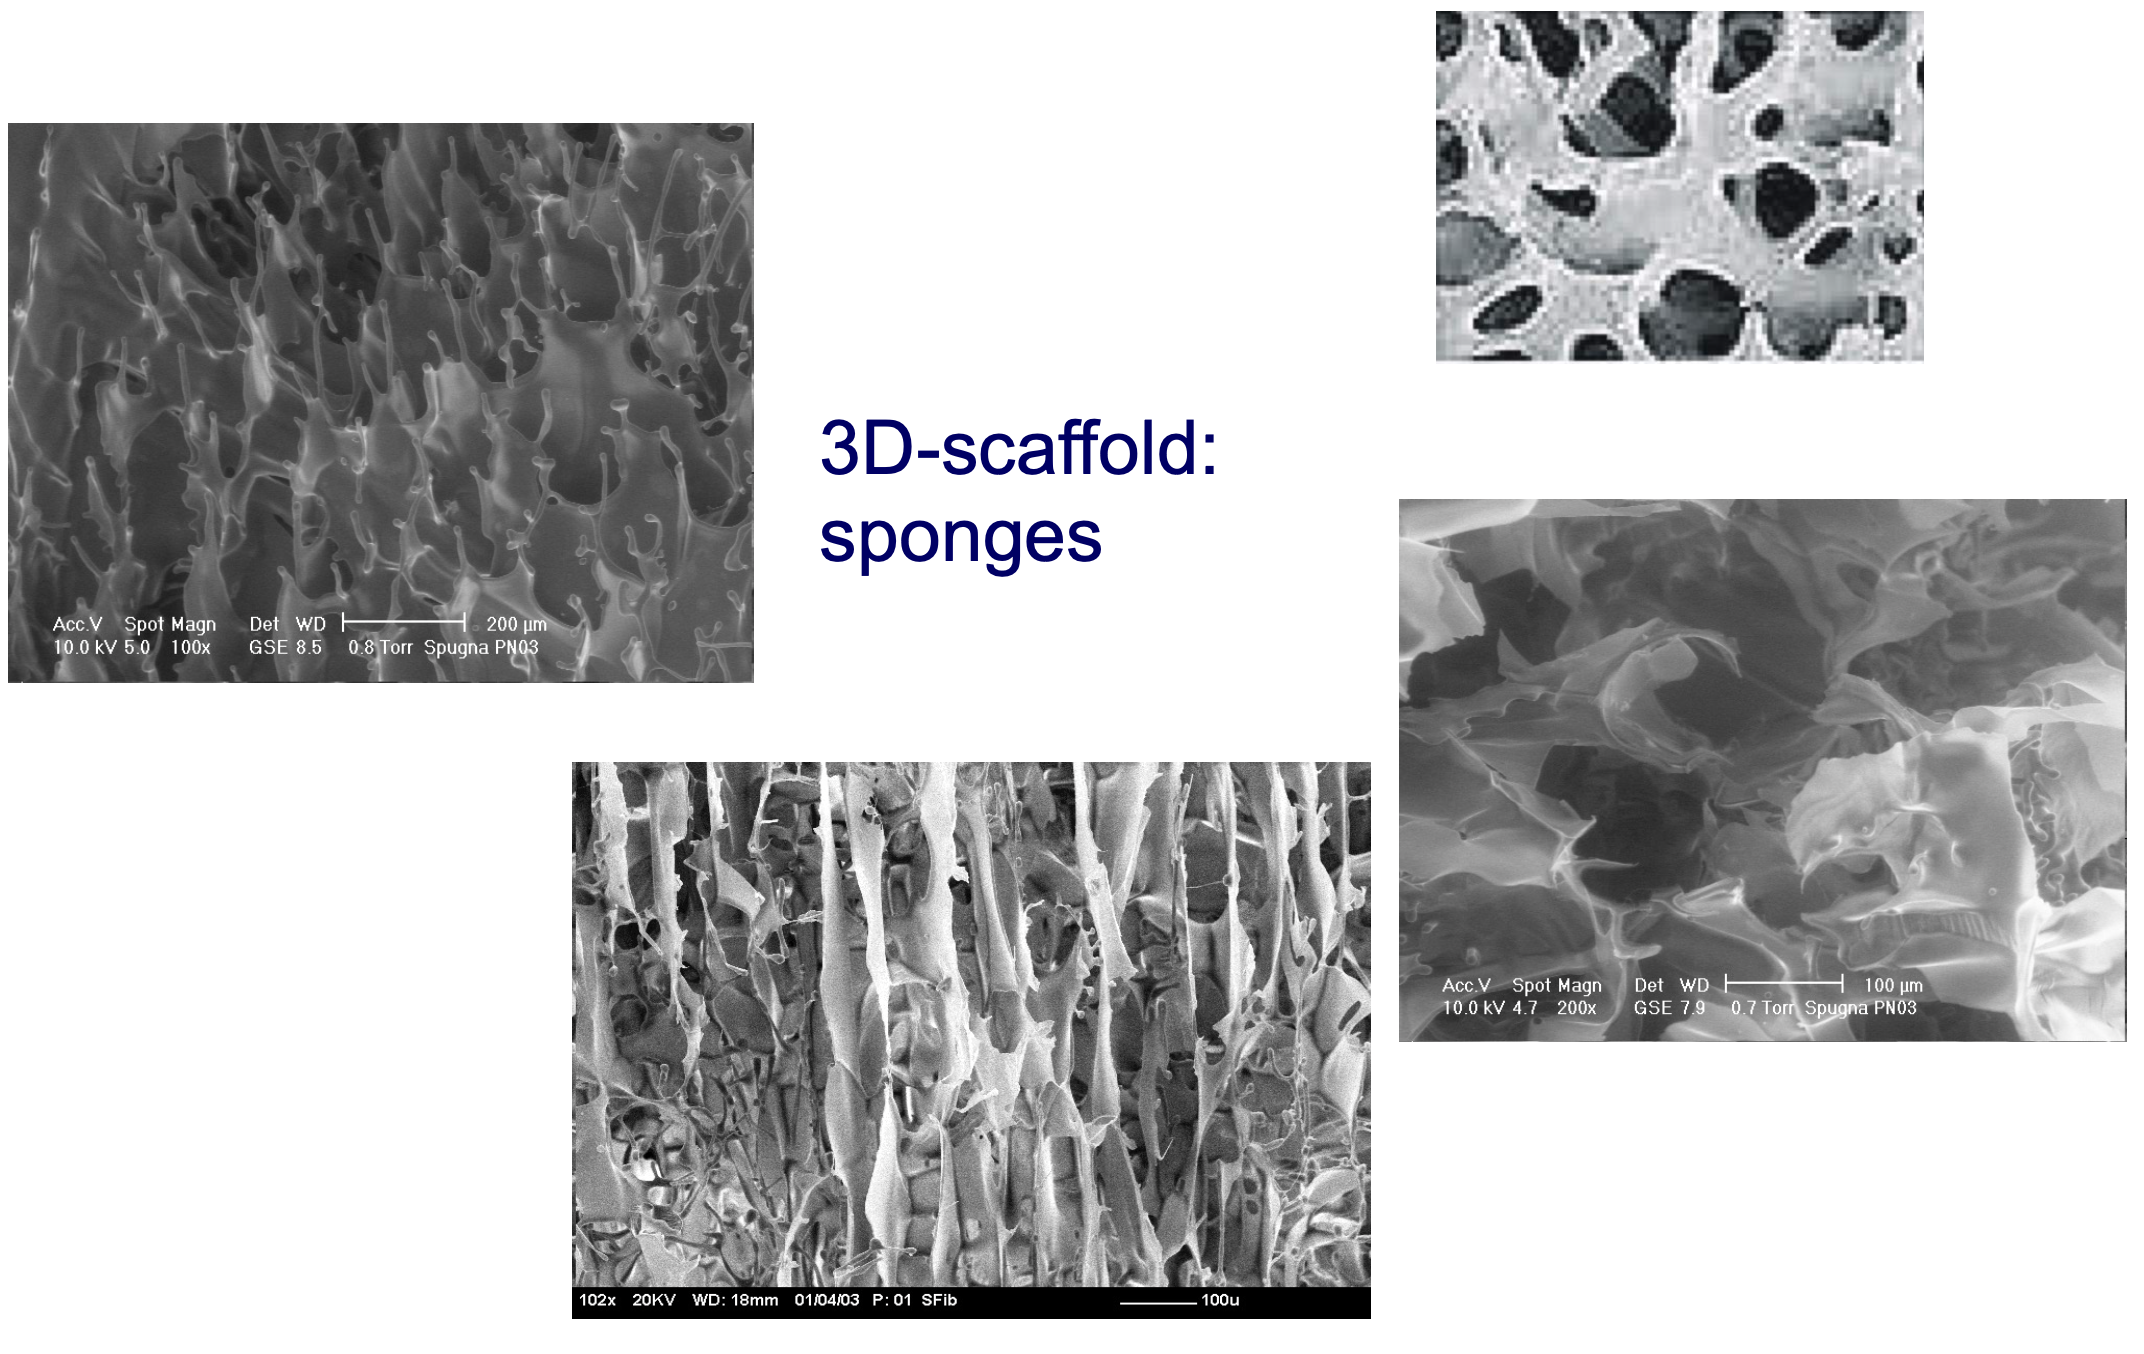
\includegraphics[width=0.5\textwidth]{sponge.png}
            \caption{\label{fig:sponge}}
            \end{figure}
        \noindent
        Fig \ref{fig:sponge} depicts the repair of trabecular bone with 3D-scaffold sponges.
        All of the images represent artificial scaffolds except the one on the top right depicts the natural sponge.
        The porosity can be oriented or random, with different geometries.
        The scaffold should promote adhesion, proliferation and migration.
        Hypoxia should be avoided, maybe with early angiogenesis.
        In vivo: in the case of bones, we have osteoblasts adhesion and migration, ECM production.
        In order to avoid hypoxia and necrotic tissue formation it is required to achieve vascularization, oxygen must be supplied to stimulate angiogenesis.
        In vitro: to test the scaffold in vivo it could be cultured in a bioreactor, a chamber with perfusion and a dynamic environment.


    \subsection{Scaffold examples}

        \subsubsection{Muscle regeneration}

        \begin{figure}[h]
            \centering
            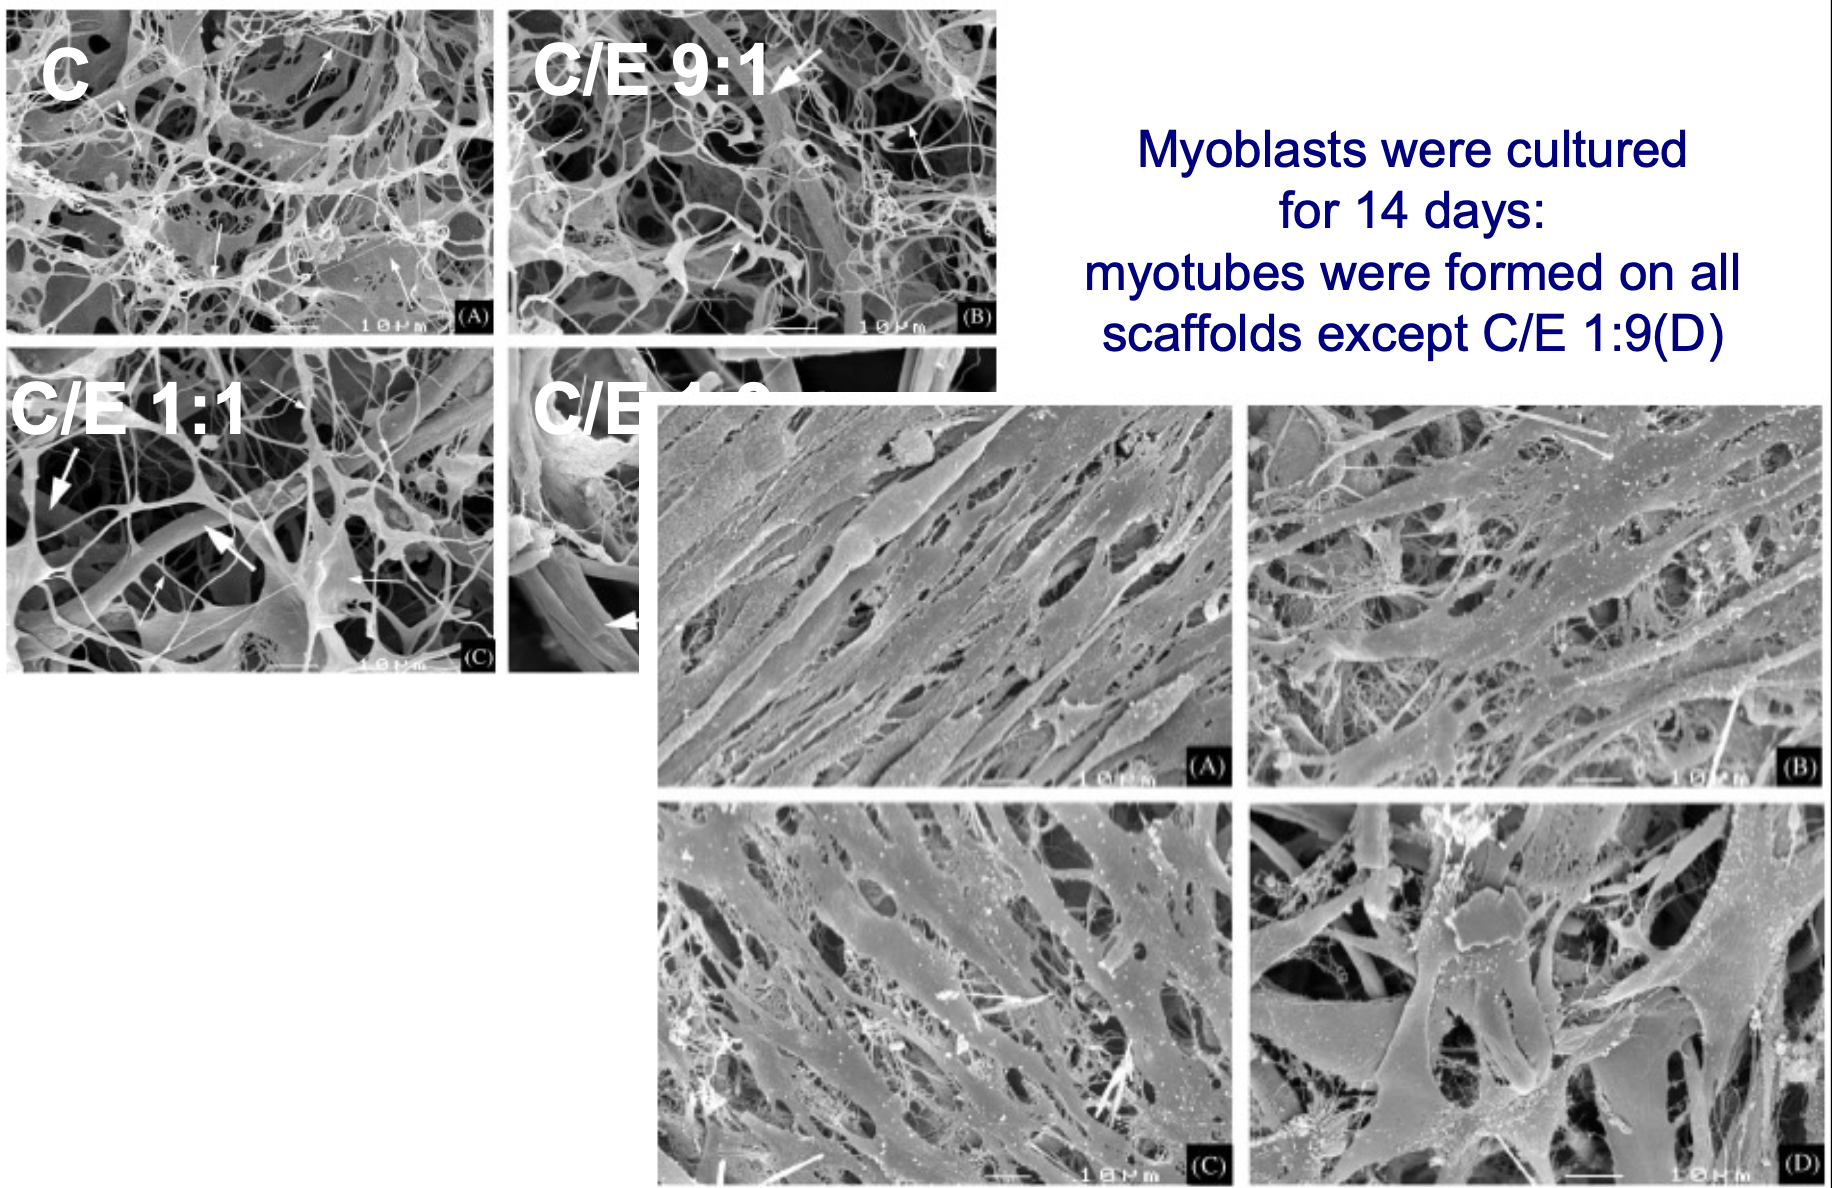
\includegraphics[width=0.5\textwidth]{myoblast.jpg}
            \caption{\label{fig:myoblast}}
        \end{figure}

        Fig \ref{fig:myoblast} depicts muscle regeneration.
        Collagen, elastin and glycosaminoglycans have been used.
        GAGs control water content and mechanical properties.
        Elastin is required for muscle elasticity and collagen for the strength.
        It is necessary to find the optimal ratio among the components.
        By changing the ratio  four different architectures are observable:

        \begin{multicols}{2}
            \begin{enumerate}
                \item C: sponge, similar to natural behaviour of collagen.
                \item C/E 9:1: big fibers starts to appear thanks to elastin.
                \item C/E 1:1: similar content to C/E 9:1.
                \item C/E 1:9: a lot of big fibers are present.
                    Pink fiber are elastin fibers.
            \end{enumerate}
        \end{multicols}

        C might not be optimal, as well as C/E 1:9, as they are quite different from biological setting.
        In vitro test: after two weeks myoblasts were cultured for 14 days and myotubes were formed on all scaffolds except C/E 1:9(D).
        A different organisation of the myotubes is observed.
        In the last example, myoblasts are not able to organise as the condition is to far from physiology.
        By considering the test, the best samples seem to be C/E 9:1 and C/E 1:1 .

        \subsubsection{Bone regeneration}

        \begin{figure}[h]
            \centering
            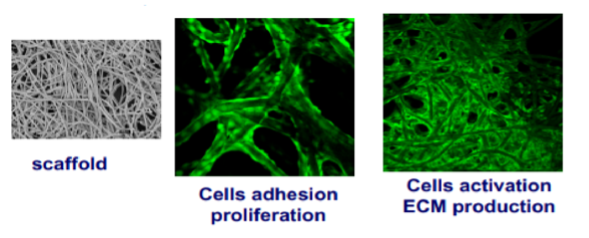
\includegraphics[width=0.6\textwidth]{3D.png}
            \caption{\label{fig:3D}}
        \end{figure}

        Figure \ref{fig:3D} represent a scaffold for bone generation and osteoblast proliferation.
        The cells, in green, are able to adhere, proliferate and migrate.
        The scaffold is then completely covered in cells.
        We then witness tissue-specific ECM production and mineralzation.
        This is a great starting point, but the degradation process of the scaffold and vascularization still need to be understood.
        In vivo vascularization can be checked performing co-culture of osteoblasts giving the angiogenesis factors and the collagenic structure for capillary network formation and endothelial cells that use empty spaces to assemble as a tube.
        It is clear that to obtain a physiological situation careful design is needed.

        \subsubsection{Polymer seeded with different cells}

        \begin{figure}[h]
            \centering
            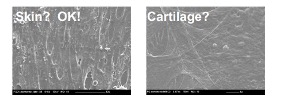
\includegraphics[width=0.6\textwidth]{sk_car.jpg}
            \caption{\label{fig:sk_car}}
        \end{figure}

        Fig \ref{fig:sk_car} depicts two film composed of the same polymers with the same architecture but seeded one with keratinocytes and the other with chondrocytes.
        The two films were completely spread.
        Cells grown in a flat dish tend to behave as individual cells or forming a monolayer, whereas cells cultured in a 3D space are more likely to assume the characteristics of a particular tissue.
        Cartilage, once grown flat, is almost impossible to shape into joints.
        The scaffold here, in the case of cartilage, is inducing the loss of the original phenotype, so it is not biocompatible.
        In the case of the skin, it is promising for biocompatibility, forming compact and well connected monolayers.

        \subsubsection{Scaffold for bone regeneration}

        \begin{figure}[h]
            \centering
            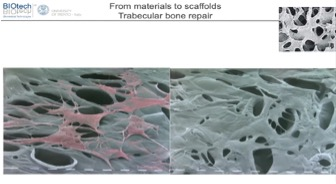
\includegraphics[width=0.5\textwidth]{bone.jpg}
            \caption{\label{fig:bone}}
        \end{figure}

        Fig \ref{fig:bone} depicts a polymer used for bone regeneration.
        In this case there is biocompatibility at all: the cells adhere to the polymer but do not migrate.
        To tackle this problem porosity should be increased.
        After few days a multi-layer structure is obtained, without migration and biocompatibility.

        \subsubsection{Seeding with suing urothelial cells}

        \begin{figure}[h]
            \centering
            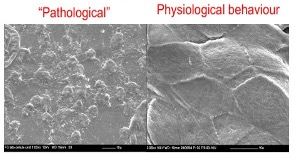
\includegraphics[width=0.5\textwidth]{suine.jpg}
            \caption{\label{fig:suine}}
        \end{figure}

        Fig \ref{fig:suine} shows suine primary urothelial cells, 6 days after seeding.
        The right image has the geometrical shape of the cells so the phenotype is ok.
        In the right image cells don’t connect and are disorganised, so they do not communicate.
        They have a more round shape, so the adherence is not good and there is no activation.

        \subsubsection{Fibroin micronet}

        \begin{figure}[h]
            \centering
            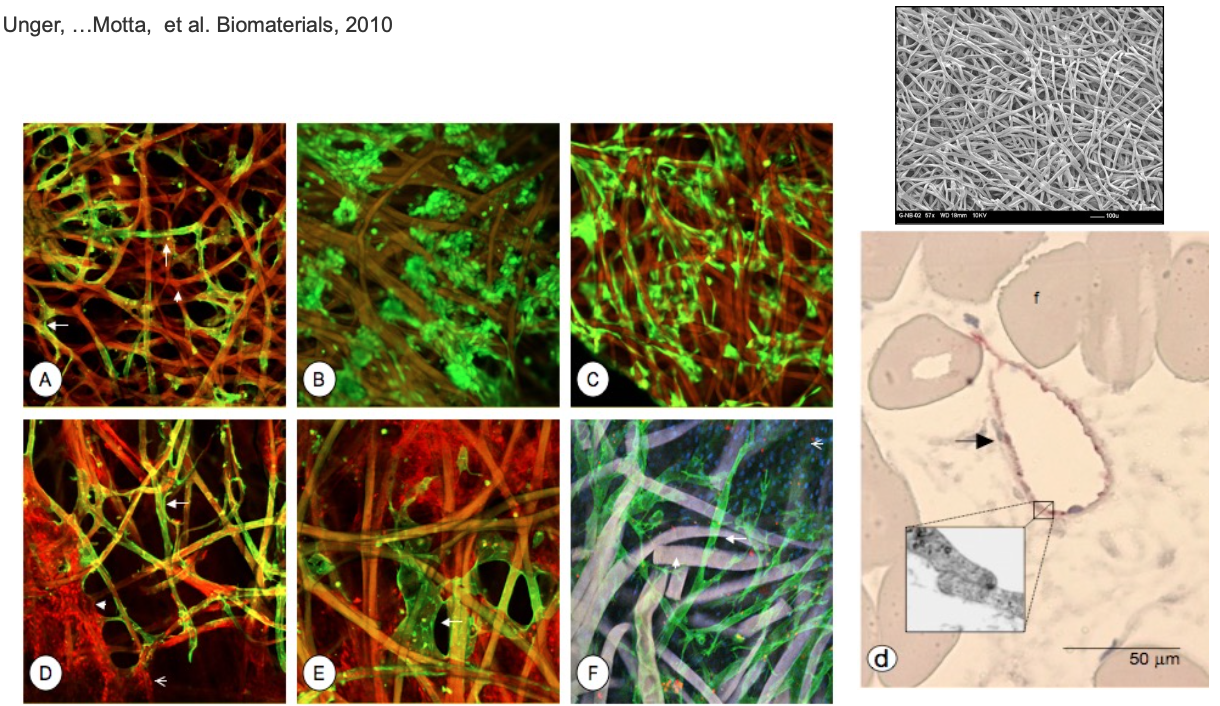
\includegraphics[width=0.5\textwidth]{fibroin}
            \caption{\label{fig:fibroin}}
        \end{figure}

        Figure \ref{fig:fibroin} represent a fibroin micronet with human microcapillary endothelial cells (HDMEC) and primary human osteoblast cells (HOS) left in co-culture for 10 days.
        The images show good result: the tubes are empty, but it is still promising.
        This tubes can be put into the scaffold and then maybe used as vessels.
        There is a need to check if the vessels connect to the circulatory system.

        \subsubsection{Pre-vascularized fibroin net}

        \begin{figure}[h]
            \centering
            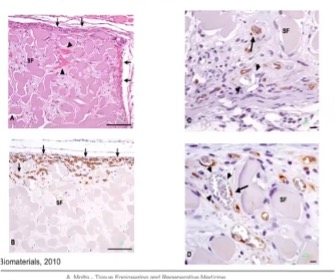
\includegraphics[width=0.5\textwidth]{osteoblast}
            \caption{\label{fig:osteoblast}}
        \end{figure}

        Figure \ref{fig:osteoblast} shows pre-vascularized fibroin net and in vivo anastomosis with host vasculature.
        Brown tubes are in vivo, and  blood cells are present and anastomise.
        The left image represent the scaffold loaded with osteoblast, incubated and then implanted.
        This shows fast angiogenesis, and only surface vessels.
        The right image represent the scaffold loaded with osteoblast and immediately implanted.
        In vitro human cells have been implanted in rat to identify the difference.
        On the right some capillaries that were produced can be seen and the absence of red blood cells can be noted.

        \subsubsection{Sponge formed from a NaCl solution}

        \begin{figure}[h]
            \centering
            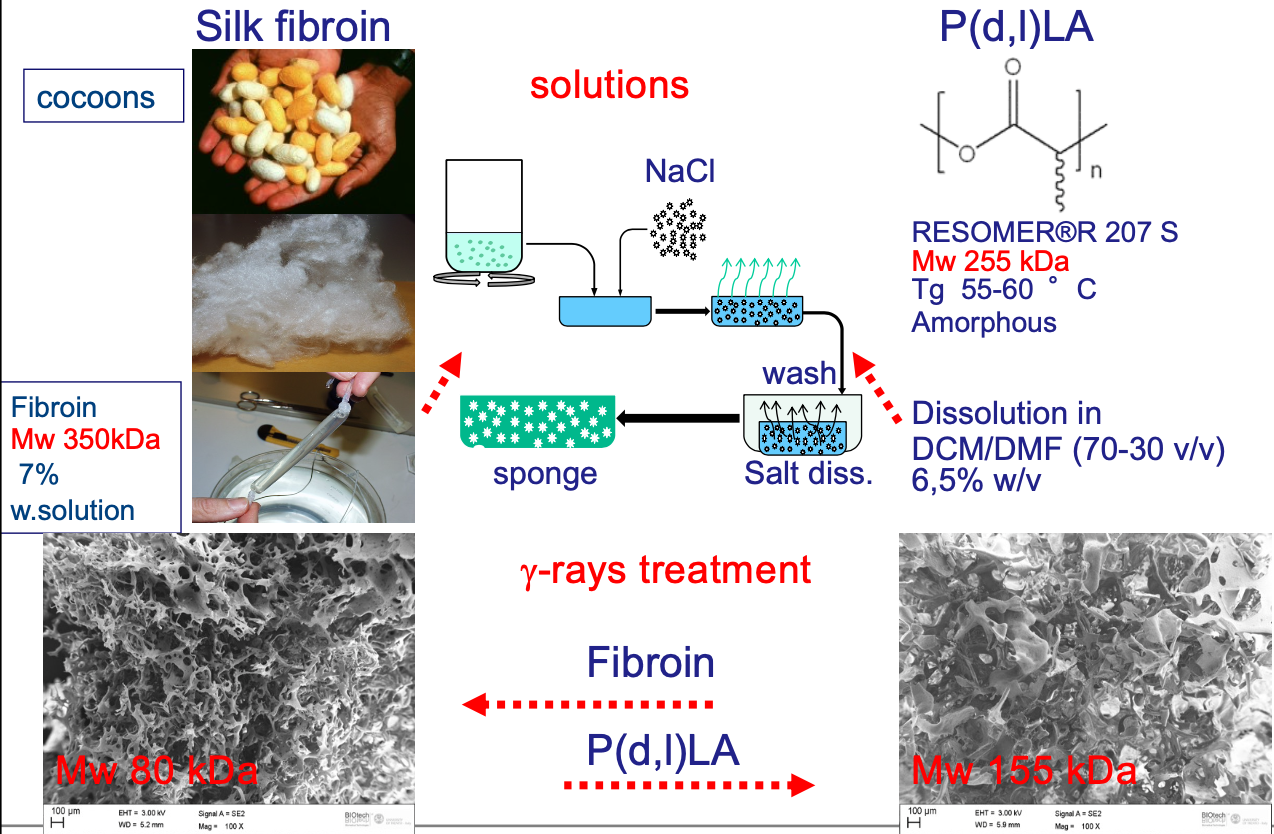
\includegraphics[width=0.5\textwidth]{salt}
            \caption{\label{fig:salt}}
        \end{figure}

        Figure \ref{fig:salt} depicts a sponge formed from salt crystals derived from a NaCl solution.
        The porosity depends on crystal size.
        Gamma rays treatment and add either silk fibroin or P(d,l)LA can be added.

        \subsubsection{Ectopic implant in rat}
        An ectopic implant is done in a sit that is not natural, in the studied case under the skin for bone.

        \begin{figure}[H]
            \centering
            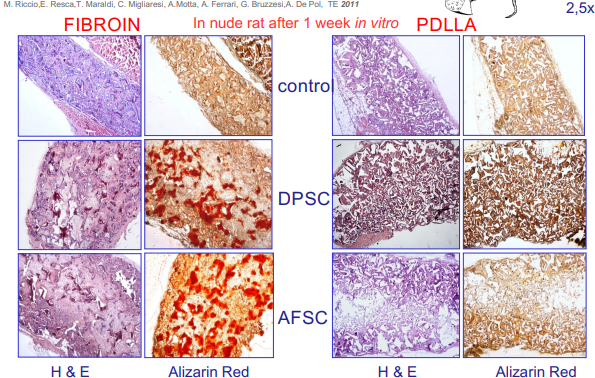
\includegraphics[width=0.5\textwidth]{implant_fibroin.png}
            \caption{\label{fig:implant_fibroin} \textbf{1. Fibroin.} In the \textbf{control} there is no red signal: no induction. There are cells (blue) but they are not infiltrated in the scaffold. There are no sign of mineralization. No osteoinduction. In \textbf{DPSC} and \textbf{AFSC} there are red nodules: it has become osteoinductive and force stem cells to become osteoblast and mineralization happens. In the H $\&$ E column a regeneration framework can be noted. \textbf{2. PDLLA} In the \textbf{control} there is not red sign so there is no induction. There are cells (blue) but they are not filtered in the scaffold. There is no mineralization or osteoinduction. In \textbf{DPSC} and \textbf{AFSC}, even in the case of pre-loaded cells there are no red signs and also there is no osteoinduction. In the center there are no cells and that suggests that the cells started to go into apoptosis.}
        \end{figure}

        \begin{figure}[H]
            \centering
            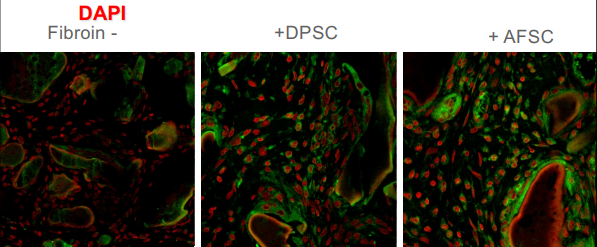
\includegraphics[width=0.5\textwidth]{fibroin_confocal.png}
            \caption{\label{fig:fibroin_confocal} In order to assess which kind of cell is working, pre-loaded cells or osteo-cells, anti-human staining can be performed.}
        \end{figure}

        \begin{figure}[H]
            \centering
            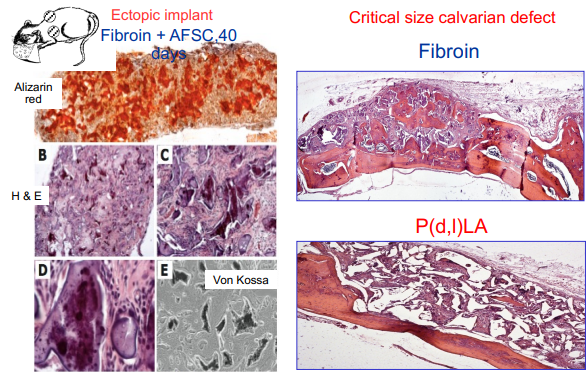
\includegraphics[width=0.5\textwidth]{intraosseous_implants.png}
            \caption{\label{fig:intraosseous_implants} \textbf{Intaosseous implants.} The \textbf{fibroin} enhance the new bone formation and supports regeneration. In \textbf{P(d,l)LA} there are lots of holes and the regenerations is not completed. It is possible to evaluate the quality of the bone and it can be seen in the fibroin it was good. There is a mixture of human and murine cells that are working together.}
        \end{figure}

        \begin{figure}[H]
            \centering
            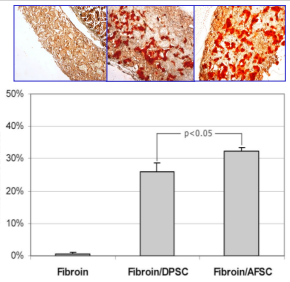
\includegraphics[width=0.5\textwidth]{mineralization.png}
            \caption{\label{fig:mineralization} \textbf{Areas of mineralization.} In the figure it is possible to see the areas of mineralization on fibroin scaffolds after 4 weeks implantation. It was calculated on 5 transversal sections cut at interval of 1 mm in the mid region of different fibroin stained by Alzarin Red. There is no mineralization in the scaffold with only fibroin, while there is mineralization in the two scaffold that present also AFSC and DPSC. There is no mineralization in the three scaffolds with PdILA.}
        \end{figure}


\section{Scaffold production technologies}

    \subsection{Cell sheet engineering}
    Cells sheet engineering is based on thermo-responsive polymers.
    They can be used in different sites like oral mucosa that present a very difficult regeneration, in periodontal ligament regeneration, but also in myocardium regeneration (as an alternative to heart transplantation).
    By transplanting single cell sheets directly to host tissues, skin, cornea, periodontal ligament, and bladder can be reconstructed.
    Additionally, the creation of co-cultured cell sheets from dishes with dual temperature-responsive domains, also allows for the re-creation of higher-order structures such as the kidney and liver.

    \begin{figure}[H]
            \centering
            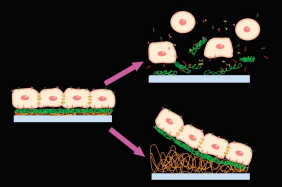
\includegraphics[width=0.5\textwidth]{cells_sheet1.png}
        \caption{\label{fig:cells_sheet1} Cell sheet harvest deposited ECM (green), as well as membrane proteins, so that confluent, monolayer cells are harvested as single cells (upper right). The temperature-responsive polymer (orange) covalently immobilized on the dish surface hydrates when the temperature is reduced, decreasing the interaction with deposited ECM. All the cells connected via cell-cell junction proteins are harvested as a single, contiguous cell sheet without the need for proteolytic enzymes.}
    \end{figure}

    \begin{figure}[H]
            \centering
            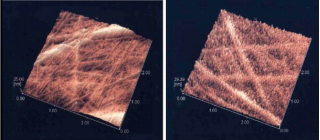
\includegraphics[width=0.5\textwidth]{cells_sheet2.png}
            \caption{\label{fig:cells_sheet2} Atomic force microscope images of temperature-responsive culture dish surfaces. Nongrafted, polystyrene culture dish surfaces (left) and poly(N-isopropylacrylamide)-grafted culture dish surfaces (right) were examined in air.}
    \end{figure}

    \begin{figure}[H]
            \centering
            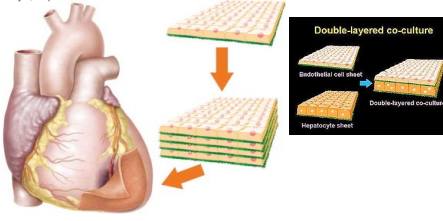
\includegraphics[width=0.5\textwidth]{cardiac_sheet.png}
            \caption{\label{fig:cardiac_sheet} Cardiac Tissue Reconstruction Based on Cell Sheet Engineering}
    \end{figure}

    \begin{figure}[H]
            \centering
            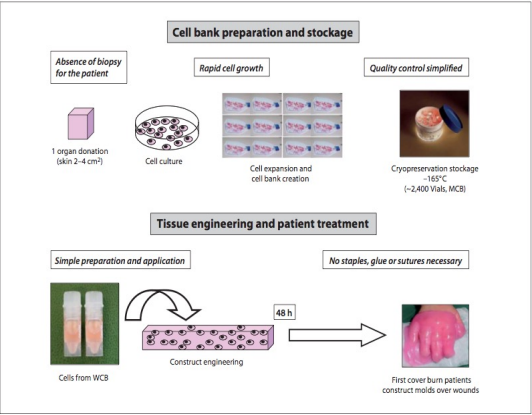
\includegraphics[width=0.5\textwidth]{cell_bank.png}
            \caption{\label{fig:cell_bank} Burnt skin}
    \end{figure}

        \subsubsection{Current challenges and strategies}

        \begin{figure}[H]
            \begin{multicols}{2}
                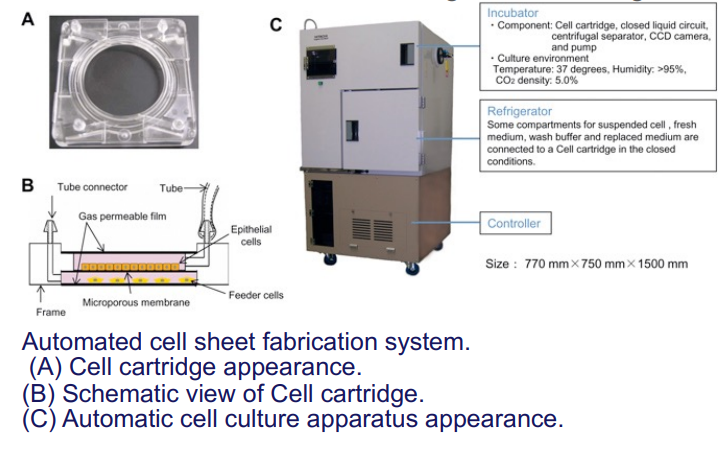
\includegraphics[width=0.5\textwidth]{strategies1.png}
                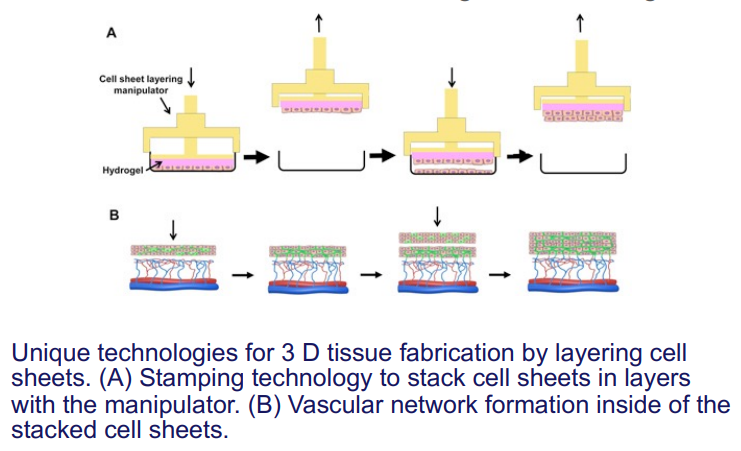
\includegraphics[width=0.5\textwidth]{strategies2.png}
                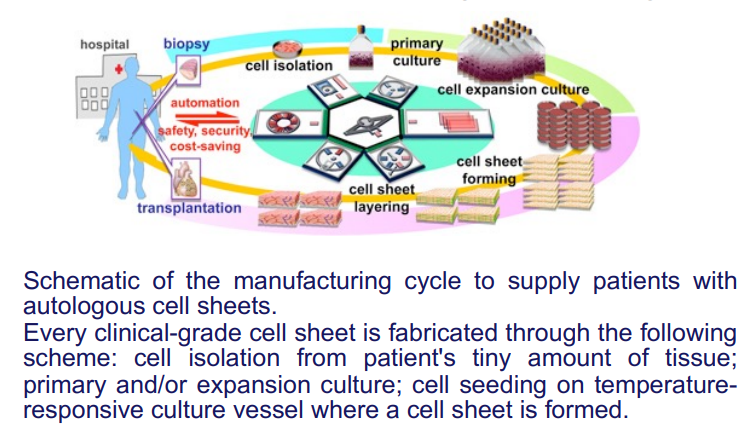
\includegraphics[width=0.5\textwidth]{strategies3.png}
                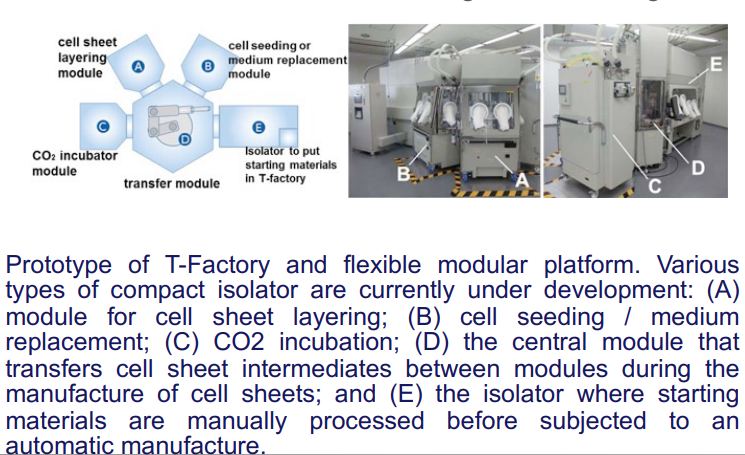
\includegraphics[width=0.5\textwidth]{strategies4.png}
            \end{multicols}
            \caption{\label{fig:strategies} Current challenges and strategies in cells sheet engineering.}
    \end{figure}

    \subsection{Cell encapsulation}
    The cell encapsulation methods consists in the entrapment of cells in microcapsules or microbeads starting from a suspension of cells in polymeric solution that can be solidified by chemical or physical methods.
    During the encapsulation the polymer cross-links by chemicals, magnetic field, light or by any other crosslinkers.

    \begin{figure}[H]
            \centering
            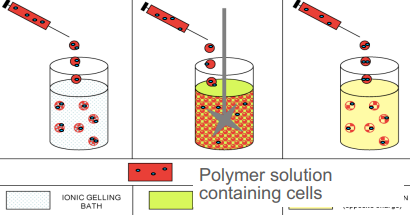
\includegraphics[width=0.5\textwidth]{encapsulation.png}
            \caption{\label{fig:encapsulation} (a) dropping the polyelectrolyte solution into a solution of small ions; (b) via a water in oil emulsification technique; and (c) complexation of oppositely charged polyelectrolytes by mixing, with additional coating procedures}.
    \end{figure}

        \subsubsection{Cell encapsulation requirements}
        Cell encapsulation requirements are:

        \begin{multicols}{2}
            \begin{itemize}
                \item The encapsulation material: a polymer should permit the free passage of nutrients and oxygen in and waste products out as well as of therapeutic protein products.
                \item Encapsulation material should prevent high Mw molecules, antibodies and other immunogenic moieties from contacting the encapsulated cells.
                \item The encapsulation material should protect cells from mechanical stresses and from the host's immune-response.
                \item The encapsulation material and method should not damage cells neither affect their behavior, as related to the desired function or application.
            \end{itemize}
        \end{multicols}

        \subsubsection{Cell encapuslation applications}
        Possible applications for cells encapsulation are drug delivery, bioartifical organs and tissue engineering.

        \begin{multicols}{2}
            \begin{itemize}
                \item The encapsulation of therapeutic cells permits the implantation of allogenic and xenogenic cells for the regulation of certain physiological processes damaged by death or senescence of host tissues.
                \item Microcapsules injected at the transplantation bed allow the release of biomolecules produced by the encapsulated cells, such as insulin produced by encapsulated $\beta$-cells for diabetes type I therapy, pro-angiogenic or anti-angiogenic growth factors to enhance or inhibit vascularization.
                \item Microencapsulated cells can be used as building blocks for the fabrication of tissues-tissue precursor in vitro or implanted in vivo for tissue regeneration.
            \end{itemize}
        \end{multicols}

\subsubsection{Short-term encapsulation effects}

\begin{figure}[H]
        \centering
        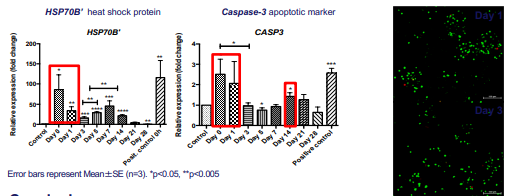
\includegraphics[width=0.5\textwidth]{short_term.png}
        \caption{\label{fig:short_term}}
\end{figure}

Short-term encapsulation effects include:

\begin{multicols}{2}
    \begin{itemize}
        \item The main function of HSP proteins consist in cells protection against apoptosis, necrosis, hypoxia or any other type of stress.
        \item Elevated co-erexpression of HSP70B' and caspase-3 genes points to mild stress conditions, and cells protection activity.
        \item The results were supported with Live/Dead test, where we can observed cell death within 48 hours after encapsulation
    \end{itemize}
\end{multicols}

\subsection{Electro-hydrodynamic jetting (EHDJ)}
In the electro-hydrodynamic systems a solution is fed through a positively charged metallic needle.
The solution reacts to the presence of the charge, generating repulsive coulombic forces on its surfaces, causing the deformation of the meniscus at the tip of the needle into a Taylor cone.
If the voltage is high enough, the electrostatic repulsion on the surface can overcome the surface tension at the apex of the liquid cone, leading to its disintegration (Rayleigh limit) and creating a jet of drops.
There are some parameters that we have to assess:

\begin{multicols}{2}
    \begin{itemize}
        \item Speed.
        \item Starting concentration of cells.
        \item Starting concentration of polymer.
        \item Type of polymer.
    \end{itemize}
\end{multicols}

Taking in consideration these parameters the final number outside of cells onto the beads can be controlled.
The quality of the concentration using a confocal microscope with live/dead staining \ref{fig:staining} can be controlled.
With this process is possible to check how many cells are alive and assess an optimal number of cells.

    \begin{figure}[H]
        \centering
        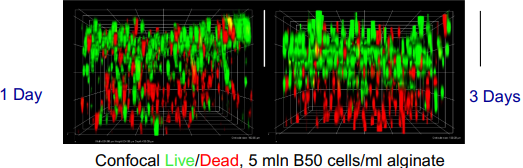
\includegraphics[width=0.5\textwidth]{staining.png}
        \caption{\label{fig:staining}}.
\end{figure}
